\documentclass[twoside]{article}

% Packages required by doxygen
\usepackage{fixltx2e}
\usepackage{calc}
\usepackage{doxygen}
\usepackage[export]{adjustbox} % also loads graphicx
\usepackage{graphicx}
\usepackage[utf8]{inputenc}
\usepackage{makeidx}
\usepackage{multicol}
\usepackage{multirow}
\PassOptionsToPackage{warn}{textcomp}
\usepackage{textcomp}
\usepackage[nointegrals]{wasysym}
\usepackage[table]{xcolor}

% Font selection
\usepackage[T1]{fontenc}
\usepackage[scaled=.90]{helvet}
\usepackage{courier}
\usepackage{amssymb}
\usepackage{sectsty}
\renewcommand{\familydefault}{\sfdefault}
\allsectionsfont{%
  \fontseries{bc}\selectfont%
  \color{darkgray}%
}
\renewcommand{\DoxyLabelFont}{%
  \fontseries{bc}\selectfont%
  \color{darkgray}%
}
\newcommand{\+}{\discretionary{\mbox{\scriptsize$\hookleftarrow$}}{}{}}

% Page & text layout
\usepackage{geometry}
\geometry{%
  a4paper,%
  top=2.5cm,%
  bottom=2.5cm,%
  left=2.5cm,%
  right=2.5cm%
}
\tolerance=750
\hfuzz=15pt
\hbadness=750
\setlength{\emergencystretch}{15pt}
\setlength{\parindent}{0cm}
\setlength{\parskip}{3ex plus 2ex minus 2ex}
\makeatletter
\renewcommand{\paragraph}{%
  \@startsection{paragraph}{4}{0ex}{-1.0ex}{1.0ex}{%
    \normalfont\normalsize\bfseries\SS@parafont%
  }%
}
\renewcommand{\subparagraph}{%
  \@startsection{subparagraph}{5}{0ex}{-1.0ex}{1.0ex}{%
    \normalfont\normalsize\bfseries\SS@subparafont%
  }%
}
\makeatother

% Headers & footers
\usepackage{fancyhdr}
\pagestyle{fancyplain}
\fancyhead[LE]{\fancyplain{}{\bfseries\thepage}}
\fancyhead[CE]{\fancyplain{}{}}
\fancyhead[RE]{\fancyplain{}{\bfseries\leftmark}}
\fancyhead[LO]{\fancyplain{}{\bfseries\rightmark}}
\fancyhead[CO]{\fancyplain{}{}}
\fancyhead[RO]{\fancyplain{}{\bfseries\thepage}}
\fancyfoot[LE]{\fancyplain{}{}}
\fancyfoot[CE]{\fancyplain{}{}}
\fancyfoot[RE]{\fancyplain{}{\bfseries\scriptsize Generated by Doxygen }}
\fancyfoot[LO]{\fancyplain{}{\bfseries\scriptsize Generated by Doxygen }}
\fancyfoot[CO]{\fancyplain{}{}}
\fancyfoot[RO]{\fancyplain{}{}}
\renewcommand{\footrulewidth}{0.4pt}
\renewcommand{\sectionmark}[1]{%
  \markright{\thesection\ #1}%
}

% Indices & bibliography
\usepackage{natbib}
\usepackage[titles]{tocloft}
\setcounter{tocdepth}{3}
\setcounter{secnumdepth}{5}
\makeindex

% Hyperlinks (required, but should be loaded last)
\usepackage{ifpdf}
\ifpdf
  \usepackage[pdftex,pagebackref=true]{hyperref}
\else
  \usepackage[ps2pdf,pagebackref=true]{hyperref}
\fi
\hypersetup{%
  colorlinks=true,%
  linkcolor=blue,%
  citecolor=blue,%
  unicode%
}

% Custom commands
\newcommand{\clearemptydoublepage}{%
  \newpage{\pagestyle{empty}\cleardoublepage}%
}

\usepackage{caption}
\captionsetup{labelsep=space,justification=centering,font={bf},singlelinecheck=off,skip=4pt,position=top}

%===== C O N T E N T S =====

\begin{document}

% Titlepage & ToC
\hypersetup{pageanchor=false,
             bookmarksnumbered=true,
             pdfencoding=unicode
            }
\pagenumbering{alph}
\begin{titlepage}
\vspace*{7cm}
\begin{center}%
{\Large tatajuba \\[1ex]\large 0.\+1 }\\
\vspace*{1cm}
{\large Generated by Doxygen 1.8.13}\\
\end{center}
\end{titlepage}
\pagenumbering{roman}
\tableofcontents
\pagenumbering{arabic}
\hypersetup{pageanchor=true}

%--- Begin generated contents ---
\section{Tatajuba source code documentation}
\label{index}\hypertarget{index}{}This is the doxyfile-\/generated documentation for \href{https://github.com/quadram-institute-bioscience/tatajuba}{\tt tatajuba}.

This documentation relates to structures, functions, etc. used by the library. 
\section{Data Structure Index}
\subsection{Data Structures}
Here are the data structures with brief descriptions\+:\begin{DoxyCompactList}
\item\contentsline{section}{\hyperlink{struct____bmc2__kstring__t}{\+\_\+\+\_\+bmc2\+\_\+kstring\+\_\+t} }{\pageref{struct____bmc2__kstring__t}}{}
\item\contentsline{section}{\hyperlink{structarg__parameters}{arg\+\_\+parameters} }{\pageref{structarg__parameters}}{}
\item\contentsline{section}{\hyperlink{structcont__hist__ptr__t}{cont\+\_\+hist\+\_\+ptr\+\_\+t} }{\pageref{structcont__hist__ptr__t}}{}
\item\contentsline{section}{\hyperlink{structcontext__histogram__struct}{context\+\_\+histogram\+\_\+struct} }{\pageref{structcontext__histogram__struct}}{}
\item\contentsline{section}{\hyperlink{structg__tract__t}{g\+\_\+tract\+\_\+t} }{\pageref{structg__tract__t}}{}
\item\contentsline{section}{\hyperlink{structg__tract__vector__struct}{g\+\_\+tract\+\_\+vector\+\_\+struct} }{\pageref{structg__tract__vector__struct}}{}
\item\contentsline{section}{\hyperlink{structgenome__set__struct}{genome\+\_\+set\+\_\+struct} }{\pageref{structgenome__set__struct}}{}
\item\contentsline{section}{\hyperlink{structgenomic__context__list__struct}{genomic\+\_\+context\+\_\+list\+\_\+struct} }{\pageref{structgenomic__context__list__struct}}{}
\item\contentsline{section}{\hyperlink{structhopo__counter__struct}{hopo\+\_\+counter\+\_\+struct} }{\pageref{structhopo__counter__struct}}{}
\item\contentsline{section}{\hyperlink{structhopo__element}{hopo\+\_\+element} }{\pageref{structhopo__element}}{}
\item\contentsline{section}{\hyperlink{structtatajuba__options__t}{tatajuba\+\_\+options\+\_\+t} }{\pageref{structtatajuba__options__t}}{}
\end{DoxyCompactList}

\section{File Index}
\subsection{File List}
Here is a list of all documented files with brief descriptions\+:\begin{DoxyCompactList}
\item\contentsline{section}{\hyperlink{context__histogram_8h}{context\+\_\+histogram.\+h} \\*Homopolymer counter }{\pageref{context__histogram_8h}}{}
\item\contentsline{section}{\hyperlink{genome__set_8h}{genome\+\_\+set.\+h} \\*Set of homopolymer counters (set of single end or paired end fastq files) }{\pageref{genome__set_8h}}{}
\item\contentsline{section}{{\bfseries kseq.\+h} }{\pageref{kseq_8h}}{}
\end{DoxyCompactList}

\section{Data Structure Documentation}
\hypertarget{struct____bmc2__kstring__t}{}\subsection{\+\_\+\+\_\+bmc2\+\_\+kstring\+\_\+t Struct Reference}
\label{struct____bmc2__kstring__t}\index{\+\_\+\+\_\+bmc2\+\_\+kstring\+\_\+t@{\+\_\+\+\_\+bmc2\+\_\+kstring\+\_\+t}}
\subsubsection*{Data Fields}
\begin{DoxyCompactItemize}
\item 
\mbox{\Hypertarget{struct____bmc2__kstring__t_a0cc4a6e0f77f6bd124651008e33d91d6}\label{struct____bmc2__kstring__t_a0cc4a6e0f77f6bd124651008e33d91d6}} 
unsigned {\bfseries l}
\item 
\mbox{\Hypertarget{struct____bmc2__kstring__t_a3db2d68492a82fd3dd63786e04ea8d1b}\label{struct____bmc2__kstring__t_a3db2d68492a82fd3dd63786e04ea8d1b}} 
unsigned {\bfseries m}
\item 
\mbox{\Hypertarget{struct____bmc2__kstring__t_ad8edcbba5c56c6f256911623e7893464}\label{struct____bmc2__kstring__t_ad8edcbba5c56c6f256911623e7893464}} 
char $\ast$ {\bfseries s}
\end{DoxyCompactItemize}


The documentation for this struct was generated from the following file\+:\begin{DoxyCompactItemize}
\item 
kseq.\+h\end{DoxyCompactItemize}

\hypertarget{structarg__parameters}{}\subsection{arg\+\_\+parameters Struct Reference}
\label{structarg__parameters}\index{arg\+\_\+parameters@{arg\+\_\+parameters}}
\subsubsection*{Data Fields}
\begin{DoxyCompactItemize}
\item 
\mbox{\Hypertarget{structarg__parameters_ac1e8a158dfe54b7fdc2f851dd5b5ffcd}\label{structarg__parameters_ac1e8a158dfe54b7fdc2f851dd5b5ffcd}} 
struct arg\+\_\+lit $\ast$ {\bfseries help}
\item 
\mbox{\Hypertarget{structarg__parameters_a198a8b119bc48b6f99b8e6ceb78f7a4d}\label{structarg__parameters_a198a8b119bc48b6f99b8e6ceb78f7a4d}} 
struct arg\+\_\+lit $\ast$ {\bfseries version}
\item 
\mbox{\Hypertarget{structarg__parameters_a0b26ccbd70ba274a29180ed1e352799d}\label{structarg__parameters_a0b26ccbd70ba274a29180ed1e352799d}} 
struct arg\+\_\+lit $\ast$ {\bfseries paired}
\item 
\mbox{\Hypertarget{structarg__parameters_ad26635309054e57c2d10e850c1764f81}\label{structarg__parameters_ad26635309054e57c2d10e850c1764f81}} 
struct arg\+\_\+int $\ast$ {\bfseries kmer}
\item 
\mbox{\Hypertarget{structarg__parameters_a0412f10a83243845b3ffd5d6d1ab1aac}\label{structarg__parameters_a0412f10a83243845b3ffd5d6d1ab1aac}} 
struct arg\+\_\+int $\ast$ {\bfseries minsize}
\item 
\mbox{\Hypertarget{structarg__parameters_a18c392342b0193fd018d637ede10e5b6}\label{structarg__parameters_a18c392342b0193fd018d637ede10e5b6}} 
struct arg\+\_\+int $\ast$ {\bfseries minread}
\item 
\mbox{\Hypertarget{structarg__parameters_a203c47970b46af9803bd713e70ce52f9}\label{structarg__parameters_a203c47970b46af9803bd713e70ce52f9}} 
struct arg\+\_\+int $\ast$ {\bfseries maxdist}
\item 
\mbox{\Hypertarget{structarg__parameters_a99c983b516df658a43b37ce3151cda42}\label{structarg__parameters_a99c983b516df658a43b37ce3151cda42}} 
struct arg\+\_\+int $\ast$ {\bfseries leven}
\item 
\mbox{\Hypertarget{structarg__parameters_a7adce1a839844f6fb0fc792dbdd78736}\label{structarg__parameters_a7adce1a839844f6fb0fc792dbdd78736}} 
struct arg\+\_\+int $\ast$ {\bfseries threads}
\item 
\mbox{\Hypertarget{structarg__parameters_adf9e1f5b281cb3c17abeeb3150ad2e25}\label{structarg__parameters_adf9e1f5b281cb3c17abeeb3150ad2e25}} 
struct arg\+\_\+file $\ast$ {\bfseries gff}
\item 
\mbox{\Hypertarget{structarg__parameters_a54cd66b63eb8e26be1371784eb778cac}\label{structarg__parameters_a54cd66b63eb8e26be1371784eb778cac}} 
struct arg\+\_\+file $\ast$ {\bfseries fna}
\item 
\mbox{\Hypertarget{structarg__parameters_a2dd93f256ed7b20ee699e8ebfcf92246}\label{structarg__parameters_a2dd93f256ed7b20ee699e8ebfcf92246}} 
struct arg\+\_\+file $\ast$ {\bfseries fastq}
\item 
\mbox{\Hypertarget{structarg__parameters_af43939056eba3201c35d1b9fc88d225b}\label{structarg__parameters_af43939056eba3201c35d1b9fc88d225b}} 
struct arg\+\_\+end $\ast$ {\bfseries end}
\item 
\mbox{\Hypertarget{structarg__parameters_a70fd68158adb5081c65c2a50734f23bd}\label{structarg__parameters_a70fd68158adb5081c65c2a50734f23bd}} 
void $\ast$$\ast$ {\bfseries argtable}
\end{DoxyCompactItemize}


The documentation for this struct was generated from the following file\+:\begin{DoxyCompactItemize}
\item 
main.\+c\end{DoxyCompactItemize}

\hypertarget{structcont__hist__ptr__t}{}\subsection{cont\+\_\+hist\+\_\+ptr\+\_\+t Struct Reference}
\label{structcont__hist__ptr__t}\index{cont\+\_\+hist\+\_\+ptr\+\_\+t@{cont\+\_\+hist\+\_\+ptr\+\_\+t}}


Collaboration diagram for cont\+\_\+hist\+\_\+ptr\+\_\+t\+:\nopagebreak
\begin{figure}[H]
\begin{center}
\leavevmode
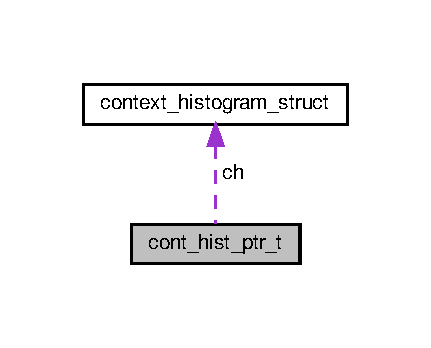
\includegraphics[width=207pt]{structcont__hist__ptr__t__coll__graph}
\end{center}
\end{figure}
\subsubsection*{Data Fields}
\begin{DoxyCompactItemize}
\item 
\mbox{\Hypertarget{structcont__hist__ptr__t_ac34cfea9f9beb575198dc84dbae23b80}\label{structcont__hist__ptr__t_ac34cfea9f9beb575198dc84dbae23b80}} 
\hyperlink{structcontext__histogram__struct}{context\+\_\+histogram\+\_\+t} {\bfseries ch}
\item 
\mbox{\Hypertarget{structcont__hist__ptr__t_af760b9184e4c3daaa6f2fc5b6df97d5a}\label{structcont__hist__ptr__t_af760b9184e4c3daaa6f2fc5b6df97d5a}} 
int {\bfseries location}
\item 
\mbox{\Hypertarget{structcont__hist__ptr__t_a03e2732c33bb949c978302a4a03f07ed}\label{structcont__hist__ptr__t_a03e2732c33bb949c978302a4a03f07ed}} 
int {\bfseries integral}
\end{DoxyCompactItemize}


The documentation for this struct was generated from the following file\+:\begin{DoxyCompactItemize}
\item 
\+\_\+\+\_\+unused.\+c\end{DoxyCompactItemize}

\hypertarget{structcontext__histogram__struct}{}\subsection{context\+\_\+histogram\+\_\+struct Struct Reference}
\label{structcontext__histogram__struct}\index{context\+\_\+histogram\+\_\+struct@{context\+\_\+histogram\+\_\+struct}}
\subsubsection*{Data Fields}
\begin{DoxyCompactItemize}
\item 
\mbox{\Hypertarget{structcontext__histogram__struct_aec81e9749874d51b633f900620f1e3e9}\label{structcontext__histogram__struct_aec81e9749874d51b633f900620f1e3e9}} 
uint64\+\_\+t $\ast$ {\bfseries context}
\item 
\mbox{\Hypertarget{structcontext__histogram__struct_a296cf58a12c2ea8604e62e2401c6c283}\label{structcontext__histogram__struct_a296cf58a12c2ea8604e62e2401c6c283}} 
int8\+\_\+t \hyperlink{structcontext__histogram__struct_a296cf58a12c2ea8604e62e2401c6c283}{base}
\begin{DoxyCompactList}\small\item\em now a vector since we store all within distance \end{DoxyCompactList}\item 
\mbox{\Hypertarget{structcontext__histogram__struct_ab51cec3be807d3531eb30864282f6dc4}\label{structcontext__histogram__struct_ab51cec3be807d3531eb30864282f6dc4}} 
char $\ast$ \hyperlink{structcontext__histogram__struct_ab51cec3be807d3531eb30864282f6dc4}{name}
\begin{DoxyCompactList}\small\item\em homopolymer base (AT or CG) \end{DoxyCompactList}\item 
\mbox{\Hypertarget{structcontext__histogram__struct_a899b6aba794f0507d258278891c3a275}\label{structcontext__histogram__struct_a899b6aba794f0507d258278891c3a275}} 
int \hyperlink{structcontext__histogram__struct_a899b6aba794f0507d258278891c3a275}{n\+\_\+context}
\begin{DoxyCompactList}\small\item\em context name is flanking kmers with tract base in the middle \end{DoxyCompactList}\item 
\mbox{\Hypertarget{structcontext__histogram__struct_aa2663ec4a4eaa334093034c756fb6fa6}\label{structcontext__histogram__struct_aa2663ec4a4eaa334093034c756fb6fa6}} 
int \hyperlink{structcontext__histogram__struct_aa2663ec4a4eaa334093034c756fb6fa6}{integral}
\begin{DoxyCompactList}\small\item\em vector size (of neighbourhood) \end{DoxyCompactList}\item 
\mbox{\Hypertarget{structcontext__histogram__struct_a553abd859781c6df2e058c9aac509d69}\label{structcontext__histogram__struct_a553abd859781c6df2e058c9aac509d69}} 
int \hyperlink{structcontext__histogram__struct_a553abd859781c6df2e058c9aac509d69}{location}
\begin{DoxyCompactList}\small\item\em sum of frequencies \end{DoxyCompactList}\item 
\mbox{\Hypertarget{structcontext__histogram__struct_a32fd0f589471b4b3457bad2519d57c0c}\label{structcontext__histogram__struct_a32fd0f589471b4b3457bad2519d57c0c}} 
int \hyperlink{structcontext__histogram__struct_a32fd0f589471b4b3457bad2519d57c0c}{coverage}
\begin{DoxyCompactList}\small\item\em genomic location(s) of context \end{DoxyCompactList}\item 
\mbox{\Hypertarget{structcontext__histogram__struct_ac6f7762a5c89e835ad78129e76b57b20}\label{structcontext__histogram__struct_ac6f7762a5c89e835ad78129e76b57b20}} 
int {\bfseries n\+\_\+tracts}
\item 
int \hyperlink{structcontext__histogram__struct_ac2bd5615e4cc759224487c986c58add3}{mode\+\_\+context\+\_\+count}
\item 
\mbox{\Hypertarget{structcontext__histogram__struct_a6387d61ff7886c0edae1d661a863b15d}\label{structcontext__histogram__struct_a6387d61ff7886c0edae1d661a863b15d}} 
int \hyperlink{structcontext__histogram__struct_a6387d61ff7886c0edae1d661a863b15d}{mode\+\_\+context\+\_\+length}
\begin{DoxyCompactList}\small\item\em frequency of reads, defining \char`\"{}best homopolymer+context\char`\"{} \end{DoxyCompactList}\item 
\mbox{\Hypertarget{structcontext__histogram__struct_a21a1dce8d58f63d65e5653cc2addc9f3}\label{structcontext__histogram__struct_a21a1dce8d58f63d65e5653cc2addc9f3}} 
int \hyperlink{structcontext__histogram__struct_a21a1dce8d58f63d65e5653cc2addc9f3}{mode\+\_\+context\+\_\+id}
\begin{DoxyCompactList}\small\item\em tract length of best homopolymer+context \end{DoxyCompactList}\item 
\mbox{\Hypertarget{structcontext__histogram__struct_a41a52c2e34beffbbab03159f0cff1f46}\label{structcontext__histogram__struct_a41a52c2e34beffbbab03159f0cff1f46}} 
int $\ast$ \hyperlink{structcontext__histogram__struct_a41a52c2e34beffbbab03159f0cff1f46}{tmp\+\_\+count}
\begin{DoxyCompactList}\small\item\em which context (from neighbourhood) has best homopolymer+context \end{DoxyCompactList}\item 
\mbox{\Hypertarget{structcontext__histogram__struct_aba1c02911d9d9c3f5a7c22866aa3ce7c}\label{structcontext__histogram__struct_aba1c02911d9d9c3f5a7c22866aa3ce7c}} 
int $\ast$ {\bfseries tmp\+\_\+length}
\item 
\mbox{\Hypertarget{structcontext__histogram__struct_ac98441e27668d56fe76a9fb3ded76ac7}\label{structcontext__histogram__struct_ac98441e27668d56fe76a9fb3ded76ac7}} 
int {\bfseries index}
\item 
\mbox{\Hypertarget{structcontext__histogram__struct_a910fe1204b22d330f4af40b88434452e}\label{structcontext__histogram__struct_a910fe1204b22d330f4af40b88434452e}} 
empfreq {\bfseries h}
\item 
\mbox{\Hypertarget{structcontext__histogram__struct_aff2efecde975d72f2b172a9edc53a125}\label{structcontext__histogram__struct_aff2efecde975d72f2b172a9edc53a125}} 
gff3\+\_\+fields {\bfseries gffeature}
\item 
\mbox{\Hypertarget{structcontext__histogram__struct_a2fb726c1bd7c20f724364e0bce705af3}\label{structcontext__histogram__struct_a2fb726c1bd7c20f724364e0bce705af3}} 
int \hyperlink{structcontext__histogram__struct_a2fb726c1bd7c20f724364e0bce705af3}{ref\+\_\+counter}
\begin{DoxyCompactList}\small\item\em could be a list (even for a single position on a single genome) but here we store first belonging \end{DoxyCompactList}\end{DoxyCompactItemize}


\subsubsection{Field Documentation}
\mbox{\Hypertarget{structcontext__histogram__struct_ac2bd5615e4cc759224487c986c58add3}\label{structcontext__histogram__struct_ac2bd5615e4cc759224487c986c58add3}} 
\index{context\+\_\+histogram\+\_\+struct@{context\+\_\+histogram\+\_\+struct}!mode\+\_\+context\+\_\+count@{mode\+\_\+context\+\_\+count}}
\index{mode\+\_\+context\+\_\+count@{mode\+\_\+context\+\_\+count}!context\+\_\+histogram\+\_\+struct@{context\+\_\+histogram\+\_\+struct}}
\paragraph{\texorpdfstring{mode\+\_\+context\+\_\+count}{mode\_context\_count}}
{\footnotesize\ttfamily int context\+\_\+histogram\+\_\+struct\+::mode\+\_\+context\+\_\+count}

values related to genome (not histogram) 

The documentation for this struct was generated from the following file\+:\begin{DoxyCompactItemize}
\item 
\hyperlink{context__histogram_8h}{context\+\_\+histogram.\+h}\end{DoxyCompactItemize}

\hypertarget{structg__tract__t}{}\subsection{g\+\_\+tract\+\_\+t Struct Reference}
\label{structg__tract__t}\index{g\+\_\+tract\+\_\+t@{g\+\_\+tract\+\_\+t}}


Collaboration diagram for g\+\_\+tract\+\_\+t\+:\nopagebreak
\begin{figure}[H]
\begin{center}
\leavevmode
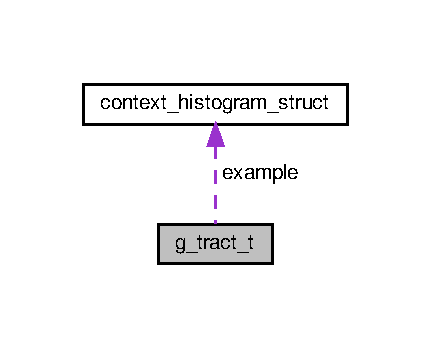
\includegraphics[width=207pt]{structg__tract__t__coll__graph}
\end{center}
\end{figure}
\subsubsection*{Data Fields}
\begin{DoxyCompactItemize}
\item 
\mbox{\Hypertarget{structg__tract__t_afd60848ec0049f7b9d4add8edf9db069}\label{structg__tract__t_afd60848ec0049f7b9d4add8edf9db069}} 
int {\bfseries location}
\item 
\mbox{\Hypertarget{structg__tract__t_a4ab5988d924fddb965685b3ec2fccd47}\label{structg__tract__t_a4ab5988d924fddb965685b3ec2fccd47}} 
int {\bfseries n\+\_\+dist}
\item 
\mbox{\Hypertarget{structg__tract__t_a8ce546dea993cb52c82f670938d1aa89}\label{structg__tract__t_a8ce546dea993cb52c82f670938d1aa89}} 
int {\bfseries lev\+\_\+distance}
\item 
\mbox{\Hypertarget{structg__tract__t_a2bf7959c381283c3ff7e6b5266f06b70}\label{structg__tract__t_a2bf7959c381283c3ff7e6b5266f06b70}} 
int {\bfseries id\+\_\+in\+\_\+concat}
\item 
\mbox{\Hypertarget{structg__tract__t_a58281833b4843de8f486e063016c0701}\label{structg__tract__t_a58281833b4843de8f486e063016c0701}} 
double $\ast$ {\bfseries tab0}
\item 
\mbox{\Hypertarget{structg__tract__t_a420632c16a20c521397aad781077427a}\label{structg__tract__t_a420632c16a20c521397aad781077427a}} 
double $\ast$ {\bfseries d1}
\item 
\mbox{\Hypertarget{structg__tract__t_a2d02b9086eee01128bdfc2997779ea54}\label{structg__tract__t_a2d02b9086eee01128bdfc2997779ea54}} 
double $\ast$ {\bfseries d2}
\item 
\mbox{\Hypertarget{structg__tract__t_ac1f6d1d94709bbbb7e2bbb0b46254b3e}\label{structg__tract__t_ac1f6d1d94709bbbb7e2bbb0b46254b3e}} 
double $\ast$ {\bfseries gentab} \mbox{[}N\+\_\+\+S\+U\+M\+M\+A\+R\+Y\+\_\+\+T\+A\+B\+L\+ES\mbox{]}
\item 
\mbox{\Hypertarget{structg__tract__t_a51eaf79b82a695bdbfd78d7937b79fb6}\label{structg__tract__t_a51eaf79b82a695bdbfd78d7937b79fb6}} 
double {\bfseries reldiff} \mbox{[}N\+\_\+\+S\+U\+M\+M\+A\+R\+Y\+\_\+\+T\+A\+B\+L\+ES\mbox{]}
\item 
\mbox{\Hypertarget{structg__tract__t_a6069f307c3bc75cb7b4091cb65c74b29}\label{structg__tract__t_a6069f307c3bc75cb7b4091cb65c74b29}} 
int {\bfseries n\+\_\+genome\+\_\+total}
\item 
\mbox{\Hypertarget{structg__tract__t_a3ddb2ee7a494bcc39607345a121cf72d}\label{structg__tract__t_a3ddb2ee7a494bcc39607345a121cf72d}} 
int {\bfseries n\+\_\+genome\+\_\+id}
\item 
\mbox{\Hypertarget{structg__tract__t_a38147086e95f9e9c9ab150dbd92942bd}\label{structg__tract__t_a38147086e95f9e9c9ab150dbd92942bd}} 
int $\ast$ {\bfseries genome\+\_\+id}
\item 
\mbox{\Hypertarget{structg__tract__t_acee1737b10a17ffb6ae86bf242eff83c}\label{structg__tract__t_acee1737b10a17ffb6ae86bf242eff83c}} 
\hyperlink{structcontext__histogram__struct}{context\+\_\+histogram\+\_\+t} {\bfseries example}
\end{DoxyCompactItemize}


The documentation for this struct was generated from the following file\+:\begin{DoxyCompactItemize}
\item 
\hyperlink{genome__set_8h}{genome\+\_\+set.\+h}\end{DoxyCompactItemize}

\hypertarget{structg__tract__vector__struct}{}\subsection{g\+\_\+tract\+\_\+vector\+\_\+struct Struct Reference}
\label{structg__tract__vector__struct}\index{g\+\_\+tract\+\_\+vector\+\_\+struct@{g\+\_\+tract\+\_\+vector\+\_\+struct}}


Collaboration diagram for g\+\_\+tract\+\_\+vector\+\_\+struct\+:\nopagebreak
\begin{figure}[H]
\begin{center}
\leavevmode
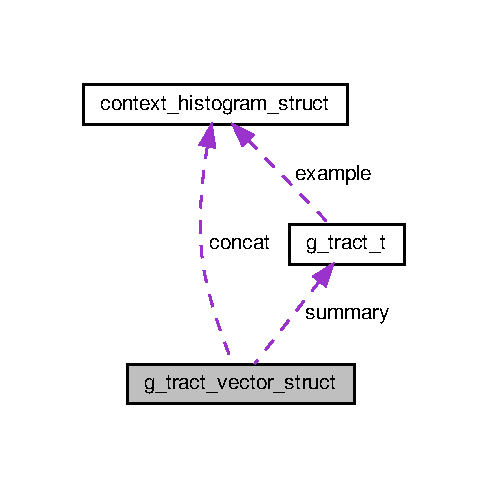
\includegraphics[width=234pt]{structg__tract__vector__struct__coll__graph}
\end{center}
\end{figure}
\subsubsection*{Data Fields}
\begin{DoxyCompactItemize}
\item 
\mbox{\Hypertarget{structg__tract__vector__struct_a10037ff5d89b6f53b216d88a103ad5e3}\label{structg__tract__vector__struct_a10037ff5d89b6f53b216d88a103ad5e3}} 
\hyperlink{structg__tract__t}{g\+\_\+tract\+\_\+t} $\ast$ {\bfseries summary}
\item 
\mbox{\Hypertarget{structg__tract__vector__struct_af0712b1af3ee47f728366e1aef7e49a9}\label{structg__tract__vector__struct_af0712b1af3ee47f728366e1aef7e49a9}} 
\hyperlink{structcontext__histogram__struct}{context\+\_\+histogram\+\_\+t} $\ast$ {\bfseries concat}
\item 
\mbox{\Hypertarget{structg__tract__vector__struct_afedcfa9a85da641f735827128d9217c9}\label{structg__tract__vector__struct_afedcfa9a85da641f735827128d9217c9}} 
int {\bfseries n\+\_\+summary}
\item 
\mbox{\Hypertarget{structg__tract__vector__struct_a90271ccb738cf5cfe6f5b732f4e5090a}\label{structg__tract__vector__struct_a90271ccb738cf5cfe6f5b732f4e5090a}} 
int {\bfseries n\+\_\+concat}
\end{DoxyCompactItemize}


The documentation for this struct was generated from the following file\+:\begin{DoxyCompactItemize}
\item 
\hyperlink{genome__set_8h}{genome\+\_\+set.\+h}\end{DoxyCompactItemize}

\hypertarget{structgenome__set__struct}{}\subsection{genome\+\_\+set\+\_\+struct Struct Reference}
\label{structgenome__set__struct}\index{genome\+\_\+set\+\_\+struct@{genome\+\_\+set\+\_\+struct}}


Collaboration diagram for genome\+\_\+set\+\_\+struct\+:\nopagebreak
\begin{figure}[H]
\begin{center}
\leavevmode
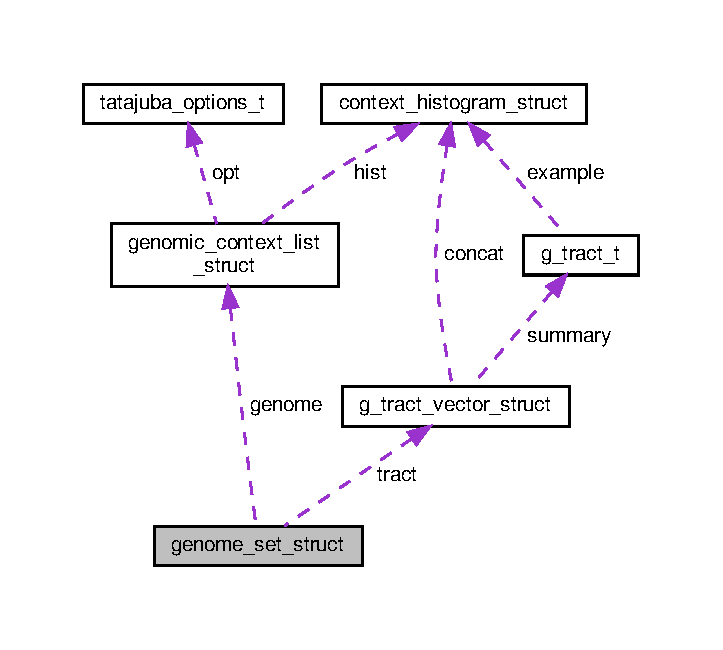
\includegraphics[width=347pt]{structgenome__set__struct__coll__graph}
\end{center}
\end{figure}
\subsubsection*{Data Fields}
\begin{DoxyCompactItemize}
\item 
\mbox{\Hypertarget{structgenome__set__struct_a78911008139357e37dc794be6d54132e}\label{structgenome__set__struct_a78911008139357e37dc794be6d54132e}} 
\hyperlink{structgenomic__context__list__struct}{genomic\+\_\+context\+\_\+list\+\_\+t} $\ast$ {\bfseries genome}
\item 
\mbox{\Hypertarget{structgenome__set__struct_a12b43be4e45be188fb908619b83d2069}\label{structgenome__set__struct_a12b43be4e45be188fb908619b83d2069}} 
\hyperlink{structg__tract__vector__struct}{g\+\_\+tract\+\_\+vector\+\_\+t} {\bfseries tract}
\item 
\mbox{\Hypertarget{structgenome__set__struct_acf6e4db81ffef1928273c9c33774e91b}\label{structgenome__set__struct_acf6e4db81ffef1928273c9c33774e91b}} 
int {\bfseries n\+\_\+genome}
\item 
\mbox{\Hypertarget{structgenome__set__struct_aca9a6a9f29b873de32db72d11bac241b}\label{structgenome__set__struct_aca9a6a9f29b873de32db72d11bac241b}} 
double {\bfseries secs} \mbox{[}3\mbox{]}
\item 
\mbox{\Hypertarget{structgenome__set__struct_ac9a18bec1d753cd0b4b15b1c9d4a480a}\label{structgenome__set__struct_ac9a18bec1d753cd0b4b15b1c9d4a480a}} 
int {\bfseries ref\+\_\+counter}
\end{DoxyCompactItemize}


The documentation for this struct was generated from the following file\+:\begin{DoxyCompactItemize}
\item 
\hyperlink{genome__set_8h}{genome\+\_\+set.\+h}\end{DoxyCompactItemize}

\hypertarget{structgenomic__context__list__struct}{}\subsection{genomic\+\_\+context\+\_\+list\+\_\+struct Struct Reference}
\label{structgenomic__context__list__struct}\index{genomic\+\_\+context\+\_\+list\+\_\+struct@{genomic\+\_\+context\+\_\+list\+\_\+struct}}


Collaboration diagram for genomic\+\_\+context\+\_\+list\+\_\+struct\+:\nopagebreak
\begin{figure}[H]
\begin{center}
\leavevmode
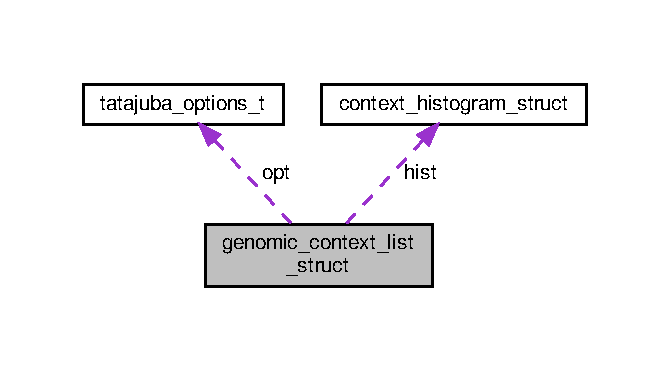
\includegraphics[width=322pt]{structgenomic__context__list__struct__coll__graph}
\end{center}
\end{figure}
\subsubsection*{Data Fields}
\begin{DoxyCompactItemize}
\item 
\mbox{\Hypertarget{structgenomic__context__list__struct_a1cb37907dc0afe1bd82be4e3a0dbf3a3}\label{structgenomic__context__list__struct_a1cb37907dc0afe1bd82be4e3a0dbf3a3}} 
\hyperlink{structcontext__histogram__struct}{context\+\_\+histogram\+\_\+t} $\ast$ {\bfseries hist}
\item 
\mbox{\Hypertarget{structgenomic__context__list__struct_a10ecf9ca3ce5e870d018b0bc2c5f0d79}\label{structgenomic__context__list__struct_a10ecf9ca3ce5e870d018b0bc2c5f0d79}} 
char $\ast$ {\bfseries name}
\item 
\mbox{\Hypertarget{structgenomic__context__list__struct_a55ae739966d02af47a49b9834bef888b}\label{structgenomic__context__list__struct_a55ae739966d02af47a49b9834bef888b}} 
\hyperlink{structtatajuba__options__t}{tatajuba\+\_\+options\+\_\+t} {\bfseries opt}
\item 
\mbox{\Hypertarget{structgenomic__context__list__struct_a4fe4f81eb544cc857a1b50fdc7f62435}\label{structgenomic__context__list__struct_a4fe4f81eb544cc857a1b50fdc7f62435}} 
int {\bfseries n\+\_\+hist}
\item 
\mbox{\Hypertarget{structgenomic__context__list__struct_ae70d8d57401f88f4e07f73a5077053dd}\label{structgenomic__context__list__struct_ae70d8d57401f88f4e07f73a5077053dd}} 
int {\bfseries coverage}
\item 
\mbox{\Hypertarget{structgenomic__context__list__struct_a7534768a48e086d0a060ecf6ccb3c5ae}\label{structgenomic__context__list__struct_a7534768a48e086d0a060ecf6ccb3c5ae}} 
int {\bfseries ref\+\_\+start}
\end{DoxyCompactItemize}


The documentation for this struct was generated from the following file\+:\begin{DoxyCompactItemize}
\item 
\hyperlink{context__histogram_8h}{context\+\_\+histogram.\+h}\end{DoxyCompactItemize}

\hypertarget{structhopo__counter__struct}{}\subsection{hopo\+\_\+counter\+\_\+struct Struct Reference}
\label{structhopo__counter__struct}\index{hopo\+\_\+counter\+\_\+struct@{hopo\+\_\+counter\+\_\+struct}}


Collaboration diagram for hopo\+\_\+counter\+\_\+struct\+:\nopagebreak
\begin{figure}[H]
\begin{center}
\leavevmode
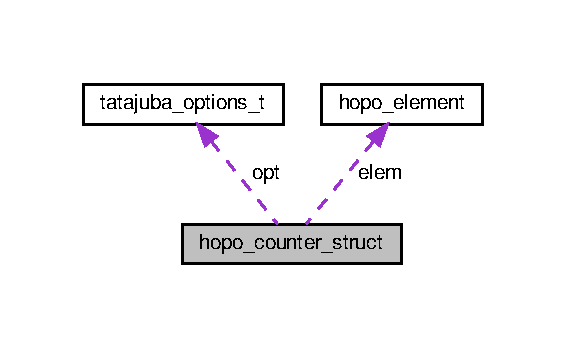
\includegraphics[width=272pt]{structhopo__counter__struct__coll__graph}
\end{center}
\end{figure}
\subsubsection*{Data Fields}
\begin{DoxyCompactItemize}
\item 
\mbox{\Hypertarget{structhopo__counter__struct_ab72daf83c1f9fbd42e9fc6f6a5e8f8ee}\label{structhopo__counter__struct_ab72daf83c1f9fbd42e9fc6f6a5e8f8ee}} 
\hyperlink{structhopo__element}{hopo\+\_\+element} $\ast$ {\bfseries elem}
\item 
\mbox{\Hypertarget{structhopo__counter__struct_ac93a5ab1f03c2e55b9f659da0a28a13b}\label{structhopo__counter__struct_ac93a5ab1f03c2e55b9f659da0a28a13b}} 
char $\ast$ {\bfseries name}
\item 
\mbox{\Hypertarget{structhopo__counter__struct_a4832bb45f09cd83f3d69f050c6df5146}\label{structhopo__counter__struct_a4832bb45f09cd83f3d69f050c6df5146}} 
int {\bfseries n\+\_\+elem}
\item 
\mbox{\Hypertarget{structhopo__counter__struct_ae17dff06dd59e5f37782c848f29543dd}\label{structhopo__counter__struct_ae17dff06dd59e5f37782c848f29543dd}} 
int {\bfseries n\+\_\+alloc}
\item 
\mbox{\Hypertarget{structhopo__counter__struct_acd0ac2cffd8871a59ceca4ed57991fad}\label{structhopo__counter__struct_acd0ac2cffd8871a59ceca4ed57991fad}} 
int {\bfseries kmer\+\_\+size}
\item 
\mbox{\Hypertarget{structhopo__counter__struct_a51908413e8871158c4f36318d44a97a8}\label{structhopo__counter__struct_a51908413e8871158c4f36318d44a97a8}} 
int {\bfseries coverage}
\item 
\mbox{\Hypertarget{structhopo__counter__struct_a7563723be42376a13e697fbe6355c9ad}\label{structhopo__counter__struct_a7563723be42376a13e697fbe6355c9ad}} 
int $\ast$ {\bfseries idx}
\item 
\mbox{\Hypertarget{structhopo__counter__struct_a25287c99ae31763306567523a94f220f}\label{structhopo__counter__struct_a25287c99ae31763306567523a94f220f}} 
int {\bfseries n\+\_\+idx}
\item 
\mbox{\Hypertarget{structhopo__counter__struct_a945977ada566dfb60d4d47d01621036d}\label{structhopo__counter__struct_a945977ada566dfb60d4d47d01621036d}} 
\hyperlink{structtatajuba__options__t}{tatajuba\+\_\+options\+\_\+t} {\bfseries opt}
\item 
\mbox{\Hypertarget{structhopo__counter__struct_a89c07bc7b8472144db54e330309145f1}\label{structhopo__counter__struct_a89c07bc7b8472144db54e330309145f1}} 
int {\bfseries ref\+\_\+counter}
\end{DoxyCompactItemize}


The documentation for this struct was generated from the following file\+:\begin{DoxyCompactItemize}
\item 
\hyperlink{context__histogram_8h}{context\+\_\+histogram.\+h}\end{DoxyCompactItemize}

\hypertarget{structhopo__element}{}\subsection{hopo\+\_\+element Struct Reference}
\label{structhopo__element}\index{hopo\+\_\+element@{hopo\+\_\+element}}
\subsubsection*{Data Fields}
\begin{DoxyCompactItemize}
\item 
\mbox{\Hypertarget{structhopo__element_a58b7710f35c288d3fa46ee630e8897c0}\label{structhopo__element_a58b7710f35c288d3fa46ee630e8897c0}} 
uint64\+\_\+t {\bfseries context} \mbox{[}2\mbox{]}
\item 
\mbox{\Hypertarget{structhopo__element_a45afc698a5f9df3a847ad8b966e11fc2}\label{structhopo__element_a45afc698a5f9df3a847ad8b966e11fc2}} 
int64\+\_\+t {\bfseries base}\+:2
\item 
\mbox{\Hypertarget{structhopo__element_a2a99a0169404bb820d71b4ed447fbc73}\label{structhopo__element_a2a99a0169404bb820d71b4ed447fbc73}} 
int64\+\_\+t {\bfseries length}\+:16
\item 
\mbox{\Hypertarget{structhopo__element_a91b12aabf5041e22d0fe177420c20b54}\label{structhopo__element_a91b12aabf5041e22d0fe177420c20b54}} 
int64\+\_\+t {\bfseries count}\+:32
\end{DoxyCompactItemize}


The documentation for this struct was generated from the following file\+:\begin{DoxyCompactItemize}
\item 
\hyperlink{context__histogram_8h}{context\+\_\+histogram.\+h}\end{DoxyCompactItemize}

\hypertarget{structtatajuba__options__t}{}\subsection{tatajuba\+\_\+options\+\_\+t Struct Reference}
\label{structtatajuba__options__t}\index{tatajuba\+\_\+options\+\_\+t@{tatajuba\+\_\+options\+\_\+t}}
\subsubsection*{Data Fields}
\begin{DoxyCompactItemize}
\item 
\mbox{\Hypertarget{structtatajuba__options__t_aef332f0338fa9ed9cf321656ed6f299a}\label{structtatajuba__options__t_aef332f0338fa9ed9cf321656ed6f299a}} 
char $\ast$ {\bfseries reference\+\_\+fasta\+\_\+filename}
\item 
\mbox{\Hypertarget{structtatajuba__options__t_a3a26c2e9f1bb0be577af3c0735139465}\label{structtatajuba__options__t_a3a26c2e9f1bb0be577af3c0735139465}} 
bool {\bfseries paired\+\_\+end}
\item 
\mbox{\Hypertarget{structtatajuba__options__t_aa047be2488f048dca8f0361e6862e87c}\label{structtatajuba__options__t_aa047be2488f048dca8f0361e6862e87c}} 
gff3\+\_\+t {\bfseries gff}
\item 
\mbox{\Hypertarget{structtatajuba__options__t_a08ac0f3e17d0395aa8c465027612208f}\label{structtatajuba__options__t_a08ac0f3e17d0395aa8c465027612208f}} 
int {\bfseries max\+\_\+distance\+\_\+per\+\_\+flank}
\item 
\mbox{\Hypertarget{structtatajuba__options__t_a172b666dc113b338535ebc2470ece295}\label{structtatajuba__options__t_a172b666dc113b338535ebc2470ece295}} 
int {\bfseries kmer\+\_\+size}
\item 
\mbox{\Hypertarget{structtatajuba__options__t_aab235ff8f2e1b66ca23e44a52e4fb087}\label{structtatajuba__options__t_aab235ff8f2e1b66ca23e44a52e4fb087}} 
int {\bfseries min\+\_\+tract\+\_\+size}
\item 
\mbox{\Hypertarget{structtatajuba__options__t_a1ac19dd3786482356f8843972e2b8ee5}\label{structtatajuba__options__t_a1ac19dd3786482356f8843972e2b8ee5}} 
int {\bfseries levenshtein\+\_\+distance}
\item 
\mbox{\Hypertarget{structtatajuba__options__t_afa3f72929d02040967cfa55ab5132eaa}\label{structtatajuba__options__t_afa3f72929d02040967cfa55ab5132eaa}} 
int {\bfseries min\+\_\+coverage}
\item 
\mbox{\Hypertarget{structtatajuba__options__t_aadcc091f814b762f8e3bec3e7fd68911}\label{structtatajuba__options__t_aadcc091f814b762f8e3bec3e7fd68911}} 
int {\bfseries n\+\_\+threads}
\end{DoxyCompactItemize}


The documentation for this struct was generated from the following file\+:\begin{DoxyCompactItemize}
\item 
\hyperlink{context__histogram_8h}{context\+\_\+histogram.\+h}\end{DoxyCompactItemize}

\section{File Documentation}
\hypertarget{context__histogram_8h}{}\subsection{context\+\_\+histogram.\+h File Reference}
\label{context__histogram_8h}\index{context\+\_\+histogram.\+h@{context\+\_\+histogram.\+h}}


homopolymer counter  


{\ttfamily \#include $<$kalign.\+h$>$}\newline
{\ttfamily \#include $<$wrapper\+\_\+bwa.\+h$>$}\newline
Include dependency graph for context\+\_\+histogram.\+h\+:\nopagebreak
\begin{figure}[H]
\begin{center}
\leavevmode
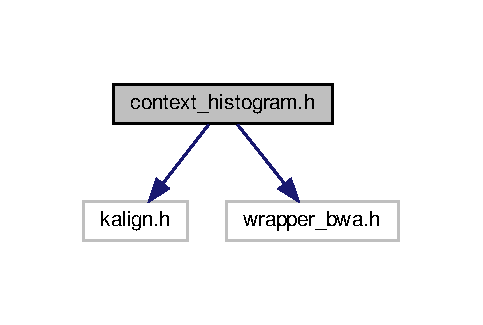
\includegraphics[width=232pt]{context__histogram_8h__incl}
\end{center}
\end{figure}
This graph shows which files directly or indirectly include this file\+:\nopagebreak
\begin{figure}[H]
\begin{center}
\leavevmode
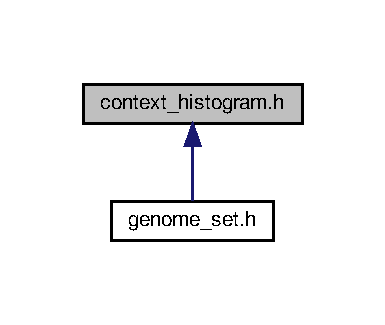
\includegraphics[width=185pt]{context__histogram_8h__dep__incl}
\end{center}
\end{figure}
\subsubsection*{Data Structures}
\begin{DoxyCompactItemize}
\item 
struct \hyperlink{structtatajuba__options__t}{tatajuba\+\_\+options\+\_\+t}
\item 
struct \hyperlink{structhopo__element}{hopo\+\_\+element}
\item 
struct \hyperlink{structhopo__counter__struct}{hopo\+\_\+counter\+\_\+struct}
\item 
struct \hyperlink{structcontext__histogram__struct}{context\+\_\+histogram\+\_\+struct}
\item 
struct \hyperlink{structgenomic__context__list__struct}{genomic\+\_\+context\+\_\+list\+\_\+struct}
\end{DoxyCompactItemize}
\subsubsection*{Typedefs}
\begin{DoxyCompactItemize}
\item 
\mbox{\Hypertarget{context__histogram_8h_acd0a87e085446a97b694d4a6f5160ebe}\label{context__histogram_8h_acd0a87e085446a97b694d4a6f5160ebe}} 
typedef struct \hyperlink{structhopo__counter__struct}{hopo\+\_\+counter\+\_\+struct} $\ast$ {\bfseries hopo\+\_\+counter}
\item 
\mbox{\Hypertarget{context__histogram_8h_a70de6dcd3ec860841c1b9a615f4d7a28}\label{context__histogram_8h_a70de6dcd3ec860841c1b9a615f4d7a28}} 
typedef struct \hyperlink{structcontext__histogram__struct}{context\+\_\+histogram\+\_\+struct} $\ast$ {\bfseries context\+\_\+histogram\+\_\+t}
\item 
\mbox{\Hypertarget{context__histogram_8h_a73614661f37cbcd280a10470ab2879de}\label{context__histogram_8h_a73614661f37cbcd280a10470ab2879de}} 
typedef struct \hyperlink{structgenomic__context__list__struct}{genomic\+\_\+context\+\_\+list\+\_\+struct} $\ast$ {\bfseries genomic\+\_\+context\+\_\+list\+\_\+t}
\end{DoxyCompactItemize}
\subsubsection*{Functions}
\begin{DoxyCompactItemize}
\item 
\mbox{\Hypertarget{context__histogram_8h_a82dde2bc7c41163ab3bfe6184fb10be8}\label{context__histogram_8h_a82dde2bc7c41163ab3bfe6184fb10be8}} 
void {\bfseries print\+\_\+tatajuba\+\_\+options} (\hyperlink{structtatajuba__options__t}{tatajuba\+\_\+options\+\_\+t} opt)
\item 
\mbox{\Hypertarget{context__histogram_8h_a15d1e8732a4f09dbaba5d0c21425ae46}\label{context__histogram_8h_a15d1e8732a4f09dbaba5d0c21425ae46}} 
\hyperlink{structhopo__counter__struct}{hopo\+\_\+counter} {\bfseries new\+\_\+or\+\_\+append\+\_\+hopo\+\_\+counter\+\_\+from\+\_\+file} (\hyperlink{structhopo__counter__struct}{hopo\+\_\+counter} hc, const char $\ast$filename, \hyperlink{structtatajuba__options__t}{tatajuba\+\_\+options\+\_\+t} opt)
\item 
\mbox{\Hypertarget{context__histogram_8h_a58485daef5d33a0eff026ca891bebd2a}\label{context__histogram_8h_a58485daef5d33a0eff026ca891bebd2a}} 
void {\bfseries del\+\_\+hopo\+\_\+counter} (\hyperlink{structhopo__counter__struct}{hopo\+\_\+counter} hc)
\item 
\mbox{\Hypertarget{context__histogram_8h_a8a6f90e88b23b34f556ab9dc0af447e4}\label{context__histogram_8h_a8a6f90e88b23b34f556ab9dc0af447e4}} 
void {\bfseries del\+\_\+context\+\_\+histogram} (\hyperlink{structcontext__histogram__struct}{context\+\_\+histogram\+\_\+t} ch)
\item 
\mbox{\Hypertarget{context__histogram_8h_a2f341d258f995ad7c996621435af4552}\label{context__histogram_8h_a2f341d258f995ad7c996621435af4552}} 
void {\bfseries print\+\_\+debug\+\_\+genomic\+\_\+context\+\_\+hist} (\hyperlink{structgenomic__context__list__struct}{genomic\+\_\+context\+\_\+list\+\_\+t} genome)
\item 
\mbox{\Hypertarget{context__histogram_8h_a323f7c5461bdc31c34121f5d6664216f}\label{context__histogram_8h_a323f7c5461bdc31c34121f5d6664216f}} 
\hyperlink{structgenomic__context__list__struct}{genomic\+\_\+context\+\_\+list\+\_\+t} {\bfseries new\+\_\+genomic\+\_\+context\+\_\+list} (\hyperlink{structhopo__counter__struct}{hopo\+\_\+counter} hc)
\item 
\mbox{\Hypertarget{context__histogram_8h_a561ea63c63259eb390370042d83b135b}\label{context__histogram_8h_a561ea63c63259eb390370042d83b135b}} 
void {\bfseries del\+\_\+genomic\+\_\+context\+\_\+list} (\hyperlink{structgenomic__context__list__struct}{genomic\+\_\+context\+\_\+list\+\_\+t} genome)
\item 
\mbox{\Hypertarget{context__histogram_8h_aeae98dd3f8f966b0869962b8d9568dce}\label{context__histogram_8h_aeae98dd3f8f966b0869962b8d9568dce}} 
void {\bfseries finalise\+\_\+genomic\+\_\+context\+\_\+hist} (\hyperlink{structgenomic__context__list__struct}{genomic\+\_\+context\+\_\+list\+\_\+t} genome)
\item 
\mbox{\Hypertarget{context__histogram_8h_a6d45ba7425bcb985195284ae97a667d3}\label{context__histogram_8h_a6d45ba7425bcb985195284ae97a667d3}} 
int {\bfseries distance\+\_\+between\+\_\+context\+\_\+histograms} (\hyperlink{structcontext__histogram__struct}{context\+\_\+histogram\+\_\+t} c1, \hyperlink{structcontext__histogram__struct}{context\+\_\+histogram\+\_\+t} c2, double $\ast$result)
\item 
\mbox{\Hypertarget{context__histogram_8h_af44006f9dd208daf9c6abfa4e18735f6}\label{context__histogram_8h_af44006f9dd208daf9c6abfa4e18735f6}} 
bool {\bfseries context\+\_\+histograms\+\_\+overlap} (\hyperlink{structcontext__histogram__struct}{context\+\_\+histogram\+\_\+t} c1, \hyperlink{structcontext__histogram__struct}{context\+\_\+histogram\+\_\+t} c2, int $\ast$distance, \hyperlink{structtatajuba__options__t}{tatajuba\+\_\+options\+\_\+t} opt)
\end{DoxyCompactItemize}
\subsubsection*{Variables}
\begin{DoxyCompactItemize}
\item 
\mbox{\Hypertarget{context__histogram_8h_a590f0f5f9ff562268b5454075f0f3783}\label{context__histogram_8h_a590f0f5f9ff562268b5454075f0f3783}} 
uint8\+\_\+t {\bfseries dna\+\_\+in\+\_\+2\+\_\+bits} \mbox{[}256\mbox{]}\mbox{[}2\mbox{]}
\item 
\mbox{\Hypertarget{context__histogram_8h_ab11f980377c45d43d6ffb9f1a9ca9b23}\label{context__histogram_8h_ab11f980377c45d43d6ffb9f1a9ca9b23}} 
char {\bfseries bit\+\_\+2\+\_\+dna} \mbox{[}$\,$\mbox{]}
\end{DoxyCompactItemize}


\subsubsection{Detailed Description}
homopolymer counter 


\hypertarget{genome__set_8h}{}\subsection{genome\+\_\+set.\+h File Reference}
\label{genome__set_8h}\index{genome\+\_\+set.\+h@{genome\+\_\+set.\+h}}


set of homopolymer counters (set of single end or paired end fastq files)  


{\ttfamily \#include \char`\"{}context\+\_\+histogram.\+h\char`\"{}}\newline
Include dependency graph for genome\+\_\+set.\+h\+:\nopagebreak
\begin{figure}[H]
\begin{center}
\leavevmode
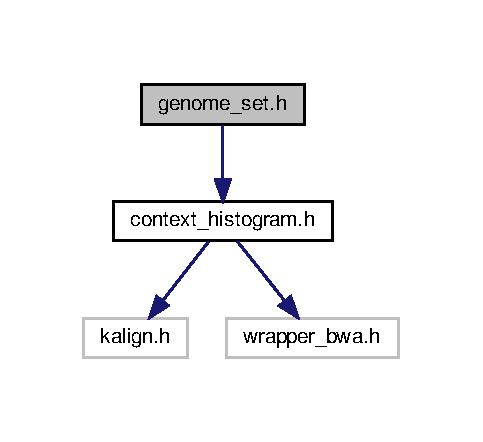
\includegraphics[width=232pt]{genome__set_8h__incl}
\end{center}
\end{figure}
\subsubsection*{Data Structures}
\begin{DoxyCompactItemize}
\item 
struct \hyperlink{structg__tract__t}{g\+\_\+tract\+\_\+t}
\item 
struct \hyperlink{structg__tract__vector__struct}{g\+\_\+tract\+\_\+vector\+\_\+struct}
\item 
struct \hyperlink{structgenome__set__struct}{genome\+\_\+set\+\_\+struct}
\end{DoxyCompactItemize}
\subsubsection*{Macros}
\begin{DoxyCompactItemize}
\item 
\mbox{\Hypertarget{genome__set_8h_a070d06a0722c1de5ca530ae5e7814b11}\label{genome__set_8h_a070d06a0722c1de5ca530ae5e7814b11}} 
\#define {\bfseries N\+\_\+\+S\+U\+M\+M\+A\+R\+Y\+\_\+\+T\+A\+B\+L\+ES}~5
\end{DoxyCompactItemize}
\subsubsection*{Typedefs}
\begin{DoxyCompactItemize}
\item 
\mbox{\Hypertarget{genome__set_8h_a355bfab53b2609a7d20ed7e706a57593}\label{genome__set_8h_a355bfab53b2609a7d20ed7e706a57593}} 
typedef struct \hyperlink{structgenome__set__struct}{genome\+\_\+set\+\_\+struct} $\ast$ {\bfseries genome\+\_\+set\+\_\+t}
\item 
\mbox{\Hypertarget{genome__set_8h_a51b20ddfc1dbf63d0670a23c901ed51f}\label{genome__set_8h_a51b20ddfc1dbf63d0670a23c901ed51f}} 
typedef struct \hyperlink{structg__tract__vector__struct}{g\+\_\+tract\+\_\+vector\+\_\+struct} $\ast$ {\bfseries g\+\_\+tract\+\_\+vector\+\_\+t}
\end{DoxyCompactItemize}
\subsubsection*{Functions}
\begin{DoxyCompactItemize}
\item 
\mbox{\Hypertarget{genome__set_8h_a0447da37499795df302faebaee748403}\label{genome__set_8h_a0447da37499795df302faebaee748403}} 
\hyperlink{structgenome__set__struct}{genome\+\_\+set\+\_\+t} {\bfseries new\+\_\+genome\+\_\+set\+\_\+from\+\_\+files} (const char $\ast$$\ast$filenames, int n\+\_\+filenames, \hyperlink{structtatajuba__options__t}{tatajuba\+\_\+options\+\_\+t} opt)
\item 
\mbox{\Hypertarget{genome__set_8h_a3a5c5b6f0ca5d431f1026bbb6e152c15}\label{genome__set_8h_a3a5c5b6f0ca5d431f1026bbb6e152c15}} 
void {\bfseries del\+\_\+genome\+\_\+set} (\hyperlink{structgenome__set__struct}{genome\+\_\+set\+\_\+t} g)
\item 
\mbox{\Hypertarget{genome__set_8h_a7e05433e507dd53090a180fb3e220f57}\label{genome__set_8h_a7e05433e507dd53090a180fb3e220f57}} 
void {\bfseries print\+\_\+selected\+\_\+g\+\_\+tract\+\_\+vector} (\hyperlink{structgenome__set__struct}{genome\+\_\+set\+\_\+t} g)
\item 
\mbox{\Hypertarget{genome__set_8h_af5775e8635374ef5825188f4c1b15053}\label{genome__set_8h_af5775e8635374ef5825188f4c1b15053}} 
void {\bfseries print\+\_\+debug\+\_\+g\+\_\+tract\+\_\+vector} (\hyperlink{structgenome__set__struct}{genome\+\_\+set\+\_\+t} g)
\end{DoxyCompactItemize}


\subsubsection{Detailed Description}
set of homopolymer counters (set of single end or paired end fastq files) 


%--- End generated contents ---

% Index
\newpage
\phantomsection
\clearemptydoublepage
\addcontentsline{toc}{section}{Index}
\printindex

\end{document}
